\documentclass[handout]{beamer}

\usepackage[utf8]{inputenc} % Language and font encoding
\usepackage[icelandic]{babel}
\usepackage[T1]{fontenc}


\usepackage{tikz}
\usepackage[listings,theorems]{tcolorbox}
\usepackage{booktabs}
\usepackage{minted} %Minted and configuration
\usemintedstyle{default}

\renewcommand{\theFancyVerbLine}{\sffamily \arabic{FancyVerbLine}}
%%%%%%%%%%%
% More math
%%%%%%%%%%%
\newcommand{\Mod}[1]{\ \text{mod}\ #1}

%%%%%%%%%%%%%%%%%%%%%%
% Beamer configuration
%%%%%%%%%%%%%%%%%%%%%%
\setbeamertemplate{navigation symbols}{}
\usecolortheme{dove}
\setbeamercolor{frametitle}{fg=white}

\usebackgroundtemplate%
{%
\vbox to \paperheight{

\includegraphics[width=\paperwidth]{Pics/hi-slide-head-2016}

\vfill
\hspace{0.5cm}
\includegraphics[width=0.3\paperwidth]{Pics/hi-von-logo}
\vspace{0.4cm}
    }%
}

\AtBeginSection[]
{
  \begin{frame}<beamer>
    \frametitle{Yfirlit}
    \tableofcontents[currentsection]
  \end{frame}
}

\setbeamerfont{frametitle}{size=\normalsize}
\addtobeamertemplate{frametitle}{}{\vspace*{0.5cm}}

%%%%%%%%%%%%%%%%%%%%%%%%%
% tcolorbox configuration
%%%%%%%%%%%%%%%%%%%%%%%%%

% Setup from: http://tex.stackexchange.com/a/43329/21638
\tcbset{%
    noparskip,
    colback=gray!10, %background color of the box
    colframe=gray!40, %color of frame and title background
    coltext=black, %color of body text
    coltitle=black, %color of title text 
    fonttitle=\bfseries,
    alerted/.style={coltitle=red, colframe=gray!40},
    example/.style={coltitle=black, colframe=green!20, colback=green!5},
}


%%%%%%%%%%%%%%%%%%%%%%%
% Further configuration
%%%%%%%%%%%%%%%%%%%%%%%
\hypersetup{colorlinks=true,pdfauthor={Eirikur Ernir Thorsteinsson},linkcolor=blue,urlcolor=blue}
\graphicspath{{./Pics/}}

\author{Eiríkur Ernir Þorsteinsson}
\institute{Háskóli Íslands}
\date{Haust 2016}

\title{Stærðfræðimynstur í tölvunarfræði}
\subtitle{Vika 12, fyrri fyrirlestur}

\begin{document}

\begin{frame}
\titlepage
\end{frame}


\section{Inngangur}

\begin{frame}{Í síðasta tíma}
\begin{itemize}
 \item Lagnet
 \item Hnútalitun
\end{itemize}
\end{frame}

\section{Tré}

\begin{frame}{Tré}
Skoðum nú sérstaka gerð neta, sem kölluð er \emph{tré}. Tvær jafngildar skilgreiningar eru:

\begin{tcolorbox}[title=Tré]
Tré (e. \emph{tree}) er samanhangandi óstefnt net án einfaldra rása.
\end{tcolorbox}

\begin{tcolorbox}[title=Tré]
Óstefnt net er tré sé til nákvæmlega einn einfaldur vegur á milli hverra tveggja hnúta í netinu.
\end{tcolorbox}

\end{frame}

\begin{frame}{Dæmi}
Netin $G_1$ og $G_2$ eru tré, en $G_3$ og $G_4$ ekki.
\begin{center}
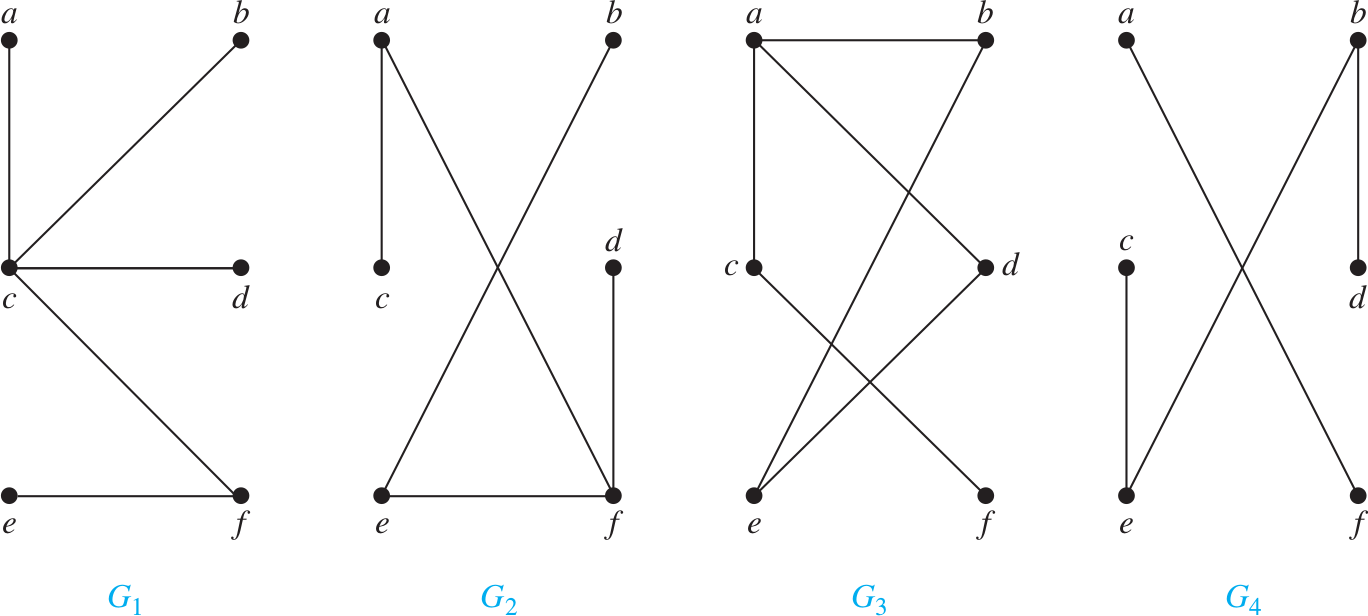
\includegraphics[width=\textwidth]{tree-not-trees}
\end{center}
\end{frame}

\begin{frame}{Skógur}
\begin{tcolorbox}[title=Skógur]
Net sem inniheldur engar einfaldar rásir er skógur (e. \emph{forest}). Skógur þarf ekki að vera samanhangandi. Hver samhengisþáttur skógar er tré.
\end{tcolorbox}
Skógur með þremur samhengisþáttum:
\begin{center}
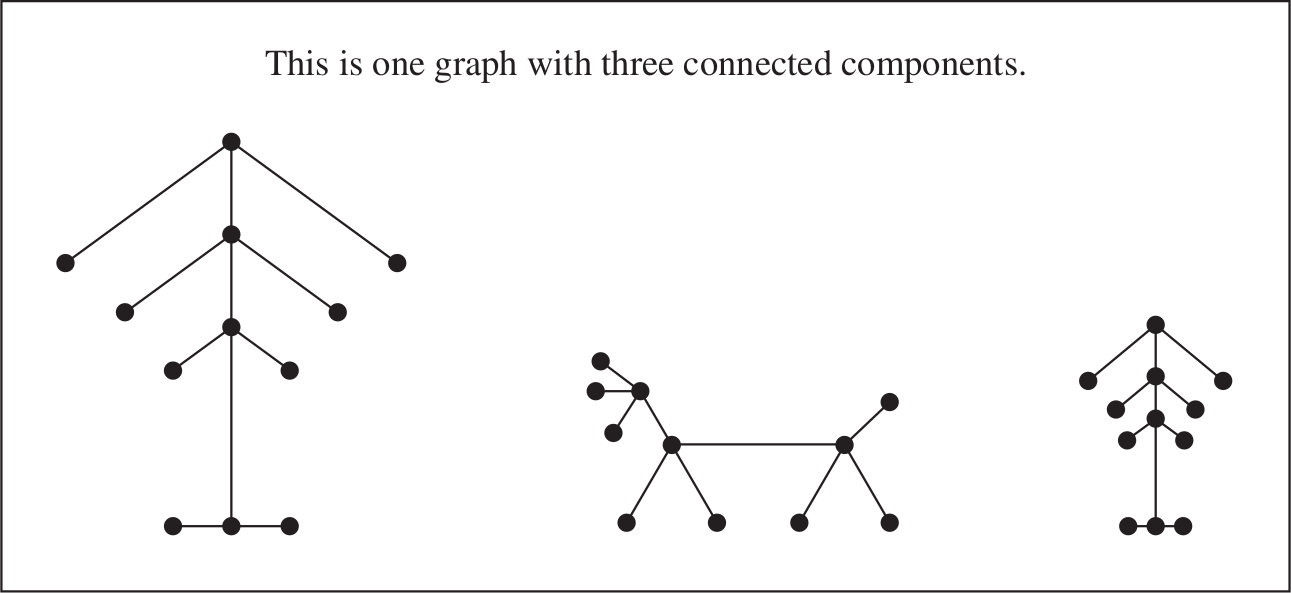
\includegraphics[width=0.8\textwidth]{tree-forest}
\end{center}
\end{frame}

\begin{frame}{Rótartré}
\begin{tcolorbox}[title=Rótartré]
Rótartré (e. \emph{rooted tree}) er tré þar sem einn hnútur hefur verið skilgreindur sem rót (e. \emph{root}). Hafi rótartré stefnu er stefna hvers leggs í átt frá rótinni.
\end{tcolorbox}
Tré $T$ og aðskilin rótartré mynduð út frá því:
\begin{center}
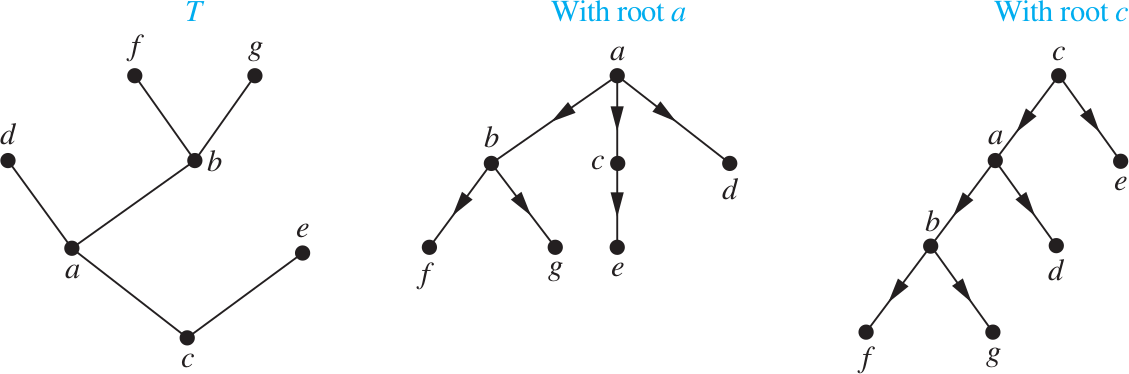
\includegraphics[width=0.8\textwidth]{tree-rooted}
\end{center}
\end{frame}

\begin{frame}{Dæmi}
\href{https://upload.wikimedia.org/wikipedia/commons/1/1b/Linux_Distribution_Timeline.svg}{``Ættarskógur'' Linux}
\end{frame}

\begin{frame}{Skráarkerfi}
\begin{center}
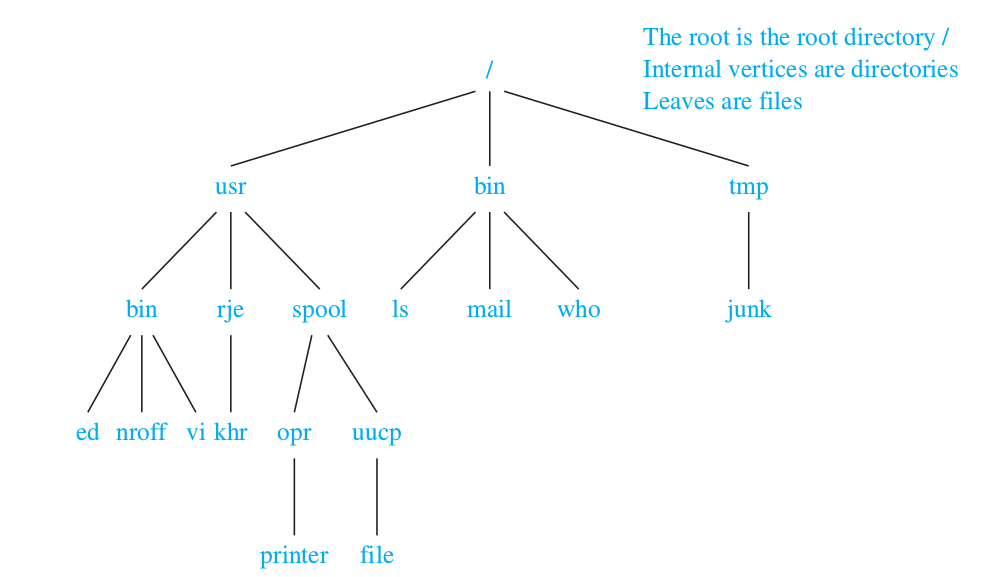
\includegraphics[width=0.7\textwidth]{tree-file-system}
\end{center}
\end{frame}

\begin{frame}{Hugtök}
\begin{itemize}
 \item Fjölmörg hugtök eru skilgreind fyrir tré og rótartré
 \item Hugtök nefnd eftir ættartengslum:
 \begin{itemize}
  \item Foreldri (e. \emph{parent}) hnúts $v$ í rótartré $T$ er eini hnúturinn $u$ í $T$ svo að $(u,v)$ sé örvaleggur
  \item Börn (e. \emph{children}) hnúts $v$ eru þeir hnútar $T$ sem hafa $v$ sem foreldri
  \item Systkin (e. \emph{siblings}) eru hnútar sem eiga sama foreldri
  \item Áar (e. \emph{ancestors}) hnúts $v$ eru þeir hnútar sem eru hluti af vegi frá rót til $v$, að $v$ sjálfum undanskildum
  \item Afkomendur (e. \emph{descendents}) hnúts $v$ eru þeir hnútar sem hafa $v$ sem áa
 \end{itemize}
\end{itemize}
\end{frame}

\begin{frame}{Hugtök}
\begin{itemize}
 \item Fleiri hugtök:
 \begin{itemize}
  \item Lauf (e. \emph{leaf}) er hnútur í tré af stigi 1
  \begin{itemize}
   \item Í rótartré má skilgreina lauf sem hnút sem á engin börn
  \end{itemize}
  \item Innri hnútur (e. \emph{internal vertex}) er hnútur í tré sem ekki er lauf
  \item Hluttré (e. \emph{subtree}) rótartrésins $T$ er rótartré $T'$ sem myndað er með hnút $a$ úr $T$ ásamt öllum afkomendum $a$ og öllum aðlægum leggjum afkomendanna
  \item Hæð (e. \emph{height}) rótartrés er fjöldi leggja í veg frá rót til laufs
  \begin{itemize}
   \item Rótin er í hæð 0
  \end{itemize}
 \end{itemize}
\end{itemize}
\end{frame}


\begin{frame}{$m$-undartré}
Rótartré sem hafa þann eiginleika að hnútarnir hafa hámarksfjölda barna koma víða við
\begin{tcolorbox}[title=$m$-undartré]
Rótartré er $m$-undartré (e. \emph{$m$-ary tree}) hafi hver innri hnútur þess að hámarki $m$ börn. Rótartré er kallað fullskipað $m$-undartré (e. \emph{full $m$-ary tree}) hafi hver innri hnútur þess nákvæmlega $m$ börn.
\end{tcolorbox}

$m$-undartré með $m = 2$ er kallað tvíundartré (e. \emph{binary tree}).
\end{frame}

\begin{frame}{Dæmi}
\begin{center}
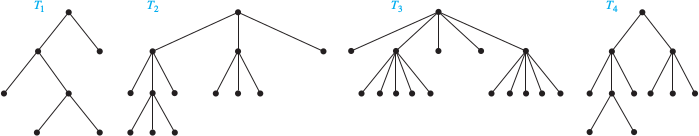
\includegraphics[width=\textwidth]{tree-full}
\end{center}
Hver þessara trjáa eru fullskipuð $m$-undartré fyrir eitthvert gildi á $m$?
\end{frame}

\begin{frame}{Röðuð rótartré}
\begin{itemize}
 \item Við getum skilgreint röðun á börn hvers hnúts í rótartré
 \begin{itemize}
  \item Getur verið mikilvægt í reikniritum
 \end{itemize}
 \item Í röðuðu tvíundartré getum við talað um ``vinstra barn'' og ``hægra barn'' einhvers hnúts
 \item Sömuleiðis getum við skilgreint ``vinstra hluttré'' og ``hægra hluttré'' fyrir einhvern hnút í rótartré
\end{itemize}
\end{frame}

\subsection{Eiginleikar trjáa}

\begin{frame}{Eiginleikar trjáa}
Við getum sett fram ýmsar staðhæfingar um samband hnúta- og leggjafjölda trjáa. Tré eru afmarkaðra fyrirbrigði en net, svo við getum sett fram sterkari staðhæfingar.

\begin{tcolorbox}
Tré með $n$ hnútum hefur $n-1$ leggi.
\end{tcolorbox}

\begin{tcolorbox}
Fullskipað $m$-undartré með $i$ innri hnúta hefur $n = mi +1$ hnúta.
\end{tcolorbox}
\end{frame}

\begin{frame}{Jafnvægi}
Oft er æskilegt að rótartré séu ``í jafnvægi''. Rótartré er í jafnvægi sé hámarksmismunur á lengd allra vega frá rót að laufi 1.

\vspace{0.5cm}
Sum eftirfarandi trjáa eru í jafnvægi:
\begin{center}
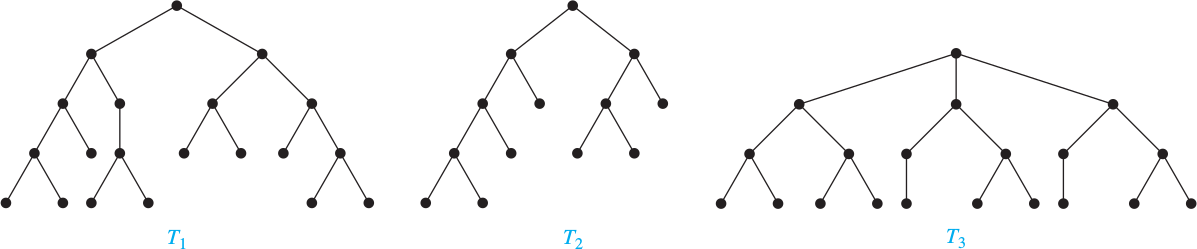
\includegraphics[width=\textwidth]{tree-balanced}
\end{center}
\pause
Það eru $T_1$ og $T_3$.
\end{frame}

\begin{frame}{Fleiri eiginleikar trjáa}
Vitum við hæð trés getum við sett skorður á laufafjöldann.
\begin{tcolorbox}
$m$-undartré af hæð $h$ hefur að hámarki $m^h$ lauf.
\end{tcolorbox}
Og enn sterkar:
\begin{tcolorbox}
$m$-undartré af hæð $h$ með $l$ lauf hefur $h \geq \lceil \log_m l \rceil$. Sé $m$-undartréð fullskipað og í jafnvægi, þá er $h = \lceil \log_m l\rceil$.
\end{tcolorbox}
\end{frame}

\section{Hagnýtingar á trjám}

\begin{frame}{Tvíleitartré}
\begin{itemize}
 \item Ein algengasta gerð verkefna sem kemur upp í tölvunarfræði er leitarverkefni
 \item Tvíleitartré (e. \emph{binary search tree}) eru mjög gagnleg þegar setja þarf upp ýmis leitarverkefni
 \item Tvíleitartré er raðað tvíundartré
 \begin{itemize}
  \item Hver hnútur er merktur með ``lykli'' (e. \emph{key})
  \begin{itemize}
   \item Við þurfum að geta borið tvo lykla saman til að athuga hvor þeirra sé stærri
  \end{itemize}
  \item Tréð er þannig upp byggt að allir lyklar í vinstra undirtré hnúts $v$ eru minni en lykill $v$, allir lyklar í hægra undirtré hnúts $v$ eru ekki minni en lykill $v$
 \end{itemize}
 \item Mjög auðvelt er að útfæra helmingunarleit sem virkar á tvíleitartré
\end{itemize}
\end{frame}

\begin{frame}{Raðað inn í tvíleitartré}
Hér eru lyklar strengir, raðað í stafrófsröð:
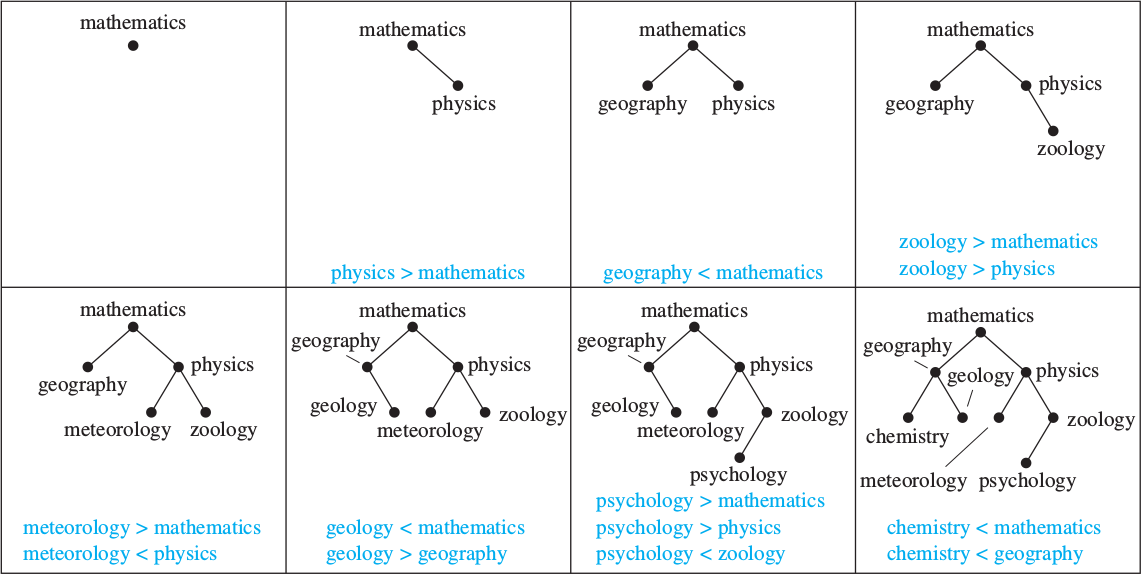
\includegraphics[width=\textwidth]{tree-subjects-search}
\end{frame}

\begin{frame}{Ákvarðanatré}
\begin{itemize}
 \item Við getum látið rótartré tákna mögulegar ákvarðanir í forriti
 \begin{itemize}
  \item Látum þá hvern hnút tákna ástand
  \item Börn hvers hnúts tákna mögulegar ákvarðanir sem hægt er að taka í því ástandi
 \end{itemize}
 \item Getum myndað einfalda ``gervigreind'' með þessum hætti
 \item Mjög svipað hugtak - leikjatré
\end{itemize}
\end{frame}

\begin{frame}{Leikjatré myllu}
\begin{center}
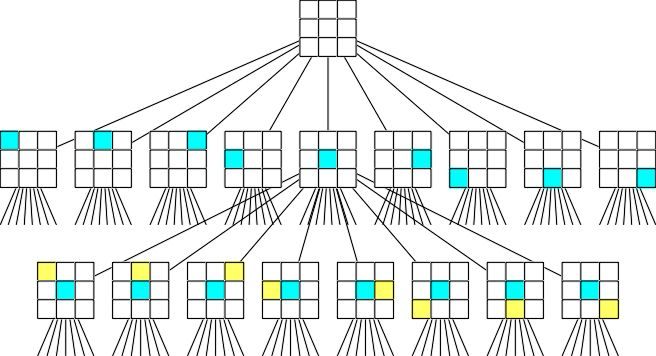
\includegraphics[width=\textwidth]{tic-tac-toe}
\end{center}
\end{frame}

\section{Fjöldi samanburða í röðun}

\begin{frame}{Fjöldi samanburða}
\begin{center}
Athugum ákvarðanatré fyrir röðun á þremur stökum $a, b$ og $c$:

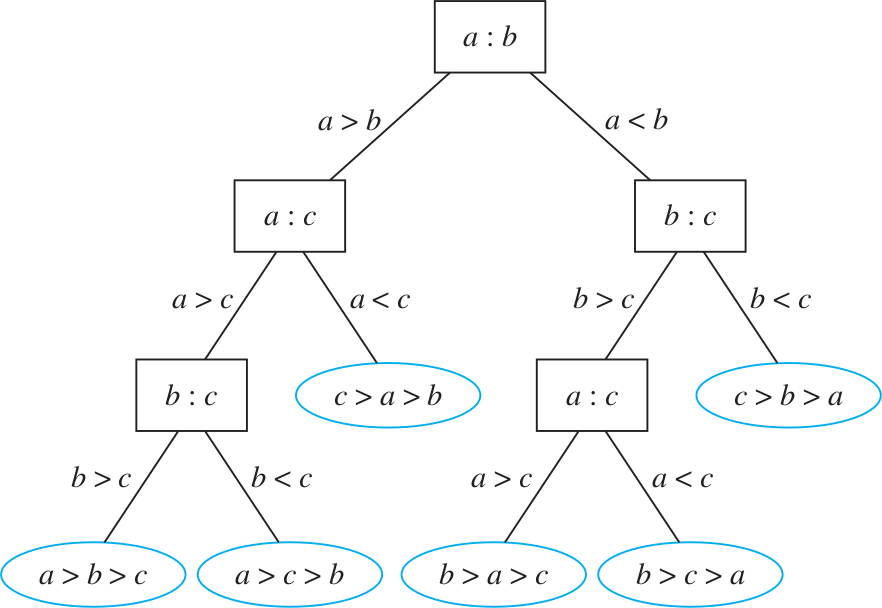
\includegraphics[width=0.7\textwidth]{tree-comparison-decision}
\end{center}
\end{frame}

\begin{frame}{Fjöldi samanburða}
\begin{itemize}
 \item Rifjum upp: Fjöldi umraðana á $n$ stökum er $n!$
 \begin{itemize}
  \item Þetta er fjöldi laufa í ákvarðanatré röðunar
 \end{itemize}
 \item Munum enn: Um $m$-undartré af hæð $h$ með $l$ lauf gildir $h \geq \lceil \log_m l\rceil$
 \begin{itemize}
  \item Afleiðing: Við þurfum $\lceil \log_m n! \rceil$ einfalda samanburði til að raða $n$ stökum
 \end{itemize}
 \item Rifjum upp: $\log n!$ er $\Theta(n \log n)$
 \begin{itemize}
  \item Afleiðing: Fjöldi samanburða sem röðunarreiknirit sem ber saman öll stökin þarf er $\Omega(n\log n)$
  \item Merge sort nær þessu!
 \end{itemize}
\end{itemize}
\end{frame}

\section{Trjáflakk}

\begin{frame}{Trjáflakk}
\begin{itemize}
 \item Tré eru skipuleg fyrirbrigði, þess vegna er auðvelt að kanna þau skipulega
 \begin{itemize}
  \item Mun auðveldara er að fara skipulega í gegnum tré en almennt net!
 \end{itemize}
 \item Skoðum sérstaklega leiðir til að kanna röðuð rótartré
 \item ``Skrifum út'' lista af gildum hnúta
 \begin{itemize}
  \item Förum alltaf sama hring í gegnum tréð, en listinn verður mismunandi eftir röð aðgerða
 \end{itemize}
\end{itemize}
\end{frame}

\begin{frame}[fragile]{Fyrirröð}
Getum skilgreint trjáflakk í fyrirröð (e. \emph{preorder traversal}).

\begin{verbatim}
stef preorder(r: hnútur í m-undartré)
  skrifa gildið í r
  fyrir b := öll börn r frá vinstri til hægri
    preorder(b)
\end{verbatim}
\end{frame}

\begin{frame}[fragile]{Miðröð}
Getum skilgreint trjáflakk í miðröð (e. \emph{inorder}).

\begin{verbatim}
stef inorder( r: hnútur í m-undartré )
  ef r er lauf þá
    skrifa gildið í r
  annars
    inorder(vinstra barn r)
    skrifa gildið í r
    fyrir b:=öll börn r nema vinstra, frá vinstri til hægri
      inorder(b)
\end{verbatim}
Miðröð kemur mjög oft fyrir, því að hún skrifar út tvíleitartré í réttri röð.
\end{frame}

\begin{frame}[fragile]{Eftirröð}
Getum skilgreint trjáflakk í eftirröð (e. \emph{postorder}).

\begin{verbatim}
stef postorder( r: hnútur í m-undartré )
  fyrir b:=öll börn r frá vinstri til hægri
    preorder(b)
  skrifa gildið í r
\end{verbatim}
\end{frame}

\begin{frame}{Samanburður}
\begin{columns}
\column{0.33\textwidth}
Fyrirröð
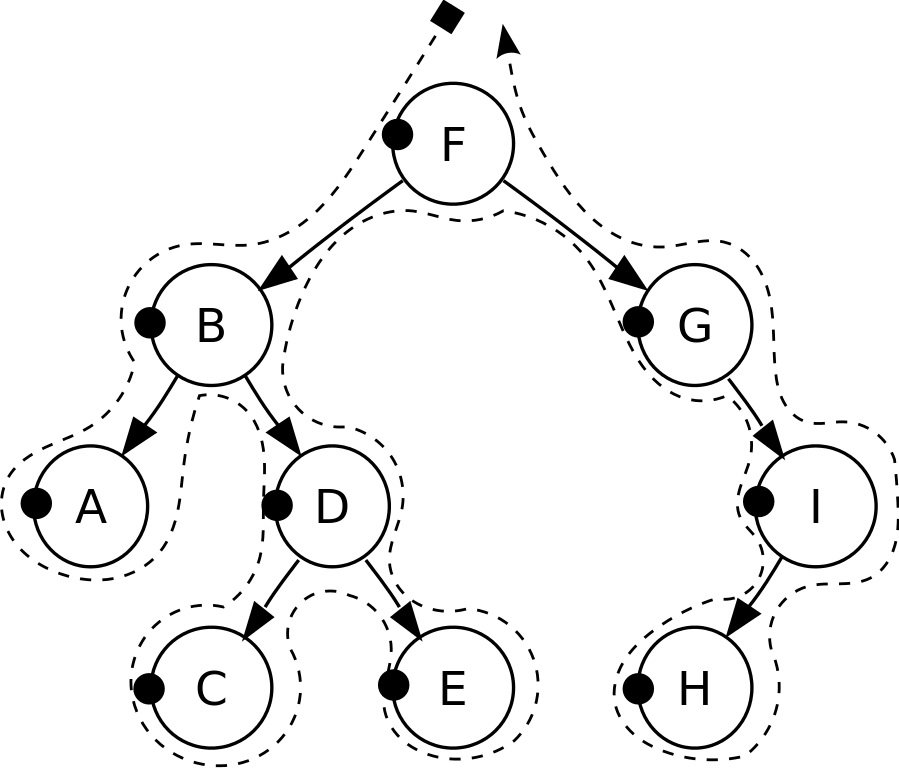
\includegraphics[width=\linewidth]{tree-preorder}
\[F, B, A, D, C, E, G, I, H\]
\column{0.33\textwidth}
Miðröð
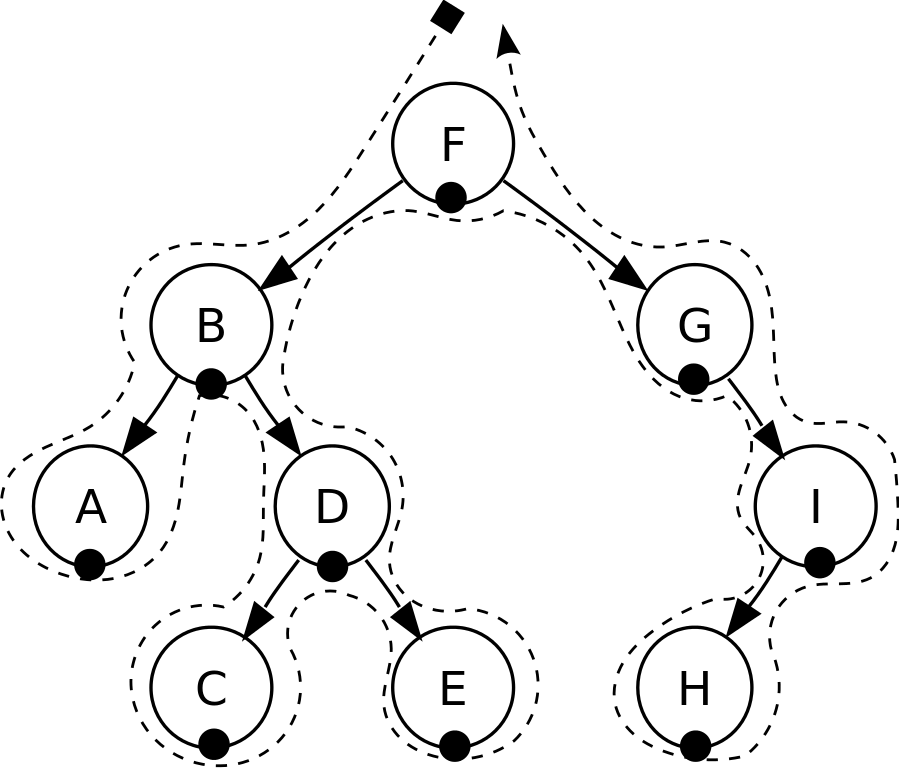
\includegraphics[width=\linewidth]{tree-inorder}
\[A, B, C, D, E, F, G, H, I\]
\column{0.33\textwidth}
Eftirröð
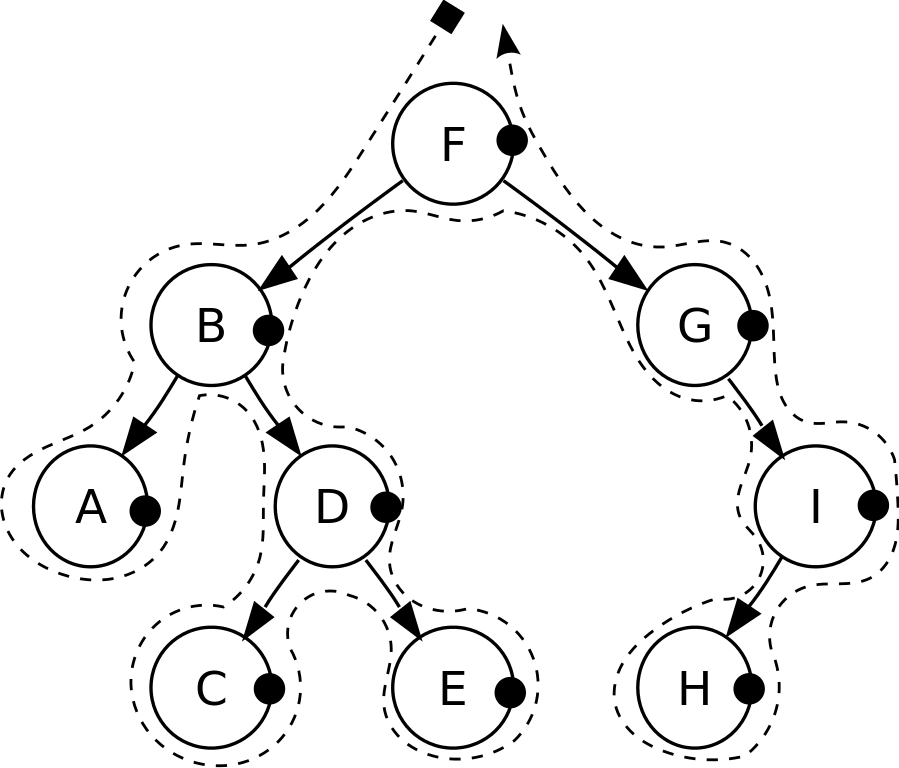
\includegraphics[width=\linewidth]{tree-postorder}
\[A, C, E, D, B, H, I, G, F\]
\end{columns}

\end{frame}



\begin{frame}{Næst}
Spanntré (11.4 og 11.5).
\end{frame}


\end{document}
